\documentclass[11pt, oneside]{article}   	% use "amsart" instead of "article" for AMSLaTeX format
\usepackage{geometry}                		% See geometry.pdf to learn the layout options. There are lots.
\geometry{a4paper}                   		% ... or a4paper or a5paper or ...letterpaper 
%\geometry{landscape}                		% Activate for rotated page geometry
%\usepackage[parfill]{parskip}    		% Activate to begin paragraphs with an empty line rather than an indent
\usepackage{graphicx}				% Use pdf, png, jpg, or eps§ with pdflatex; use eps in DVI mode
								% TeX will automatically convert eps --> pdf in pdflatex		
\usepackage{amssymb}
\DeclareGraphicsExtensions{.pdf,.png,.jpg}
\graphicspath{ {images/} }

\usepackage{hyperref}
\usepackage{subcaption}
\usepackage{amsmath}


\title{Connecting Nutrition, Health and Environment }
\author{Perla Troncoso Rey, Wiktor Jurkowski, Earlham Institute}
\date{26 - 27 January 2017}	 % Activate to display a given date or no date

\begin{document}
\maketitle

\tableofcontents

\listoffigures
\listoftables


\part{Part I}

\section{Introduction to the data}

Some details

\subsection{Exploring the expression data}



\subsubsection{Principal Component Analysis}

Principal Component Analysis, PCA, is a mathematical technique that is used to explore data, specially high-dimensional data. PCA is a method of extracting some of the most important trends in high-dimensional data.

Example of data is shown in \autoref{fig:ExpressionData}

\begin{figure}[!h]
	\centering
	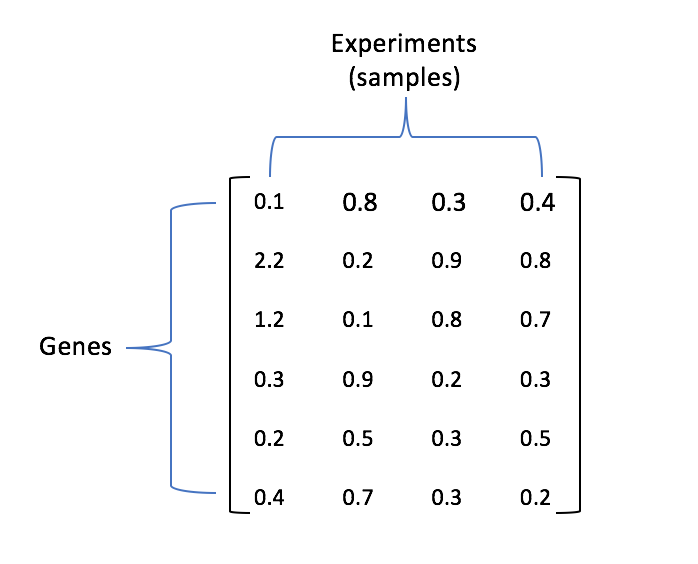
\includegraphics[width=0.7\textwidth]{example_expression_data}
	\caption{Example of expression data with samples across the columns and individual genes down the rows.}
	\label{fig:ExpressionData}
\end{figure}

high dimensionality: 
as many dimensions as number of genes
The result of each experiment can be thought as a kind of space, where each each feature is a coordinate in the space. 
there are typically thousands of genes 
the structure of pattern in the data extends to all the dimensions 

Tools to perform PCA:

\begin{itemize}
   \item MATLAB
   \item R
\end{itemize}


How it works:


The mean represents the average of the values in the data:

\begin{equation}
   \bar{{\bf X}} = \frac{1}{n} \sum_{i=1}^{n} x_i 
\end{equation}

The variance provides the the spread of the data:

\begin{equation}
   \text{Var} ({\bf X}) = \sigma^2  = \frac{1}{n-1} \sum_{i=1}^{n} ( x_i -  \bar{{\bf X}})^2
\end{equation}


For example, \ref{fig:MeanVariance} show two distribution with the same mean but different variance. 

\begin{figure}[!h]
	\centering
	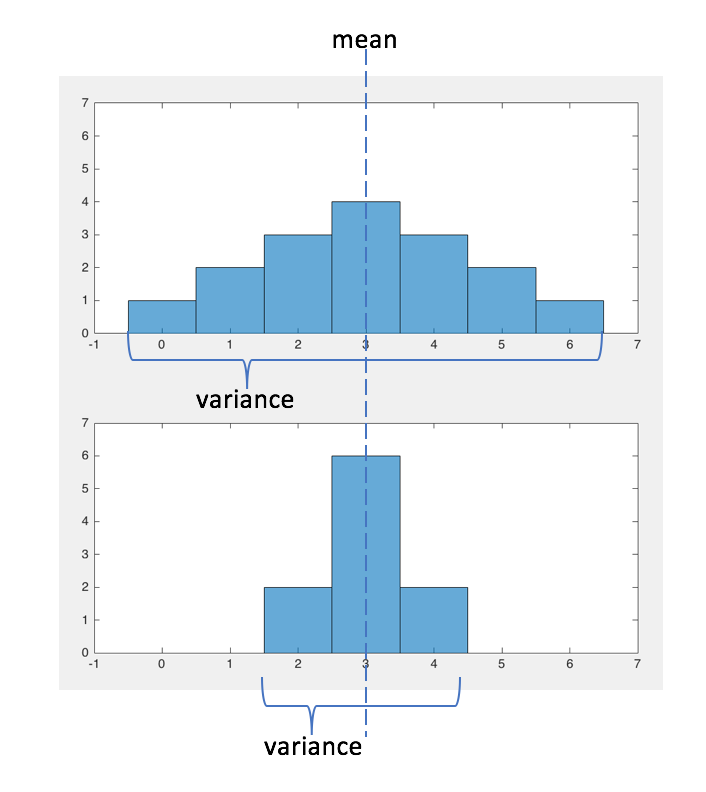
\includegraphics[width=0.7\textwidth]{same-mean_different-variance}
	\caption{Two distributions with the same mean but different variance.}
	\label{fig:MeanVariance}
\end{figure}


(i.e. the data points are at the same location but with a different strength. So the third statistic we'll need is the covariance)

The covariance represents the degree of co-dependence of two variables, i.e., it measures the co-dependency of two variables, given by:

\begin{equation}
   \text{Cov} ({\bf X}, {\bf Y}) = \frac{1}{n-1} \sum_{i=1}^{n} (x_i - \bar{ {\bf X}}) (y_i - \bar{ {\bf Y}})
\end{equation}

Increases with increasing co-dependency and variance. Just as the variance measures the degree to which a set of data varies, the co-variance is a measure of the way two sets of data vary together.

\begin{equation}
   \text{Cov} ({\bf X}, {\bf X}) = \text{Var}({\bf X})
\end{equation}

The covariance also increases in magnitude as the variance of each of the two datasets increases.


\begin{figure}[!h]
	\centering
	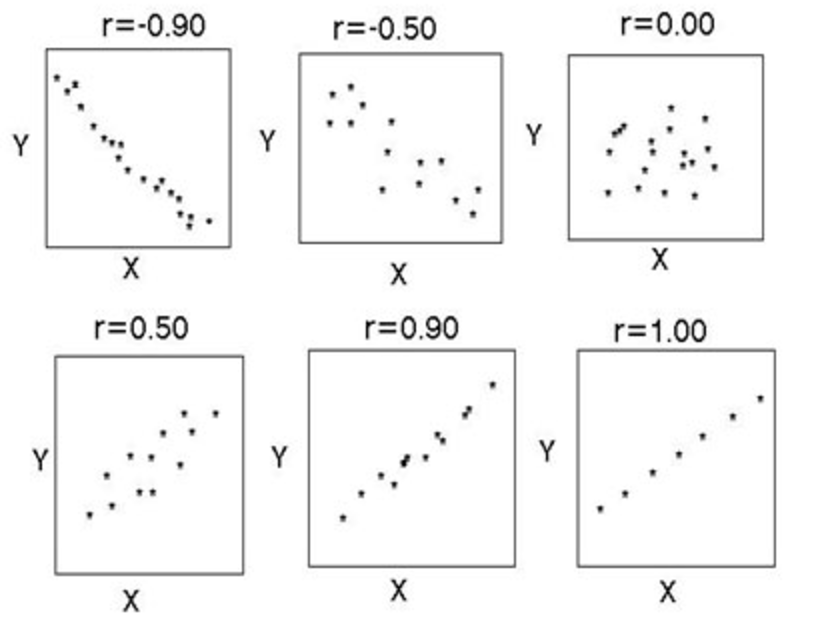
\includegraphics[width=0.7\textwidth]{examples-correlation}
	\caption{Examples of correlation}
	\label{fig:MeanVariance}
\end{figure}



Coordinate transformations

- Two dimensional space described by coordinates (i.e. a point in space described by $x_1$ and $y_1$ such that ${\bf v} = [x_1, y_1]$).

xxxxxxxxxxxxxx


PCA benefits (merits)

- A powerful tool to visualise high dimensional data 

- Shows quantified difference among observations

- Used to assess data quality and discover relationships between data points


Example 1:

PCA Plot of gene expression data 

Each dot is a gene expression from a sample in each category (class) from a patient, and is coloured by its sub-type

The three axis are the three principal components 
and the numbers represent the percentage of variance that is captured by each component

The first component captures the most variance, whereas the second and third capture only a small percentage

Dots of the same subtype tend to cluster together which means that samples of the same subtype have similar transcritption profiles.


The distance on the dots on each axis should not be treated equally (as each component captures a different percentage of variance). difference on the first component should be taken into more consideration.



Example 2: Random data

Simulated gene expression data by random numbers

This is how a random dataset would look like in a PCA plot:

- dots of different classes mix all together

- the first three components capture almost equal and small variance

- from the plot once would conclude that the different subtypes are not distinct from each other or that subtype has no influence on tumor cell transcriptome



DATA PREPARATION

- Use microarray gene expression data as an example

- Gene expression data is usually stored in a tab delimited text file. The extension of such files could be .csv, .soft, .xls(x), etc. Use Excell of Sublimetext to open and preview the file.

- Gene expression values must be normalised before PCA plotting.


PCA

- We need to transpose the matrix because the function requires the rows of the input matrix to be observations and the columns variable, which means rows to be the gene expression profiles and columns to be the genes.

- There are three outputs to the function:

1. The first output is the coefficient matrix (not used here!)

2. The second output is the scores, which are the transformed coordinates by PCA.

3. The third output, pca variance, stores how much variance each component captures.


Looking into detail on the outputs:

- The first several components capture most variance of the data.

- The score matrix has the same arrangement as expression matrix, which are rows as gene expression profiles and columns are genes. We pick the first three columns, namely the first three components. The first component will be the x-axis, the second to be the y-axis and the third component to be the z-axis.

Running PCA

%in R using prcomp from the stats package
%
%Computing the Principal Components
%
%load the data
%
%normalise data
%log transform (as suggested by xxxxx]
%log.data <- log
%
%Call prcomp with center and scale equal to TRUE to standardise the variables prior PCA



PCA Plot using MultiPEN

Parameters:

gene expression data

groups



\subsubsection{Hierarchical Clustering}

\subsection{Interaction Network}
\subsubsection{Compile the network with Cytoscape}


\part{Part II}
\section{Ranking genes (Feature Selection)} 

Feature selection with MultiPEN from expression leves and network 


\section{Pathway Analysis}

Objective

Steps

Input data
A list of ranked genes. For this session we will use the rankings from feature selection in ExampleOutputs\/MultiPEN\-Rankings\_lambda0.0001.txt.

To run the R script type in the terminal:

Rscript enrichmentGO.R ../ExampleOutputs/MultiPEN\-Rankings\_lambda0.0001.txt output/



%Example to create a list
%List:
%\begin{itemize}
%	\item item 1
%	\item item 2		
%\end{itemize}


%Example to enumerate a list
%\begin{enumerate}	
%	\item enumerated item
%	\item another item
%\end{enumerate}


%Figure resference \autoref{fig:volcanoplot}). 
%
%\begin{figure}[!h]
%	\centering
%	\includegraphics[width=\textwidth]{VolcanoMatrix}
%	\caption{Matrix of volcano plots explore genes that differ significantly between pairs of conditions}
%	\label{fig:volcanoplot}
%\end{figure}

%figure with subfigures
%\begin{figure}[!h]
%	\centering
%	\begin{subfigure}{.3\textwidth}
%		\includegraphics[width=\textwidth]{MAPlotEPS1_8_EPS2_8}
%		\caption{MA for EPS1 and EPS2, 8 hours}
%		\label{fig:MAPlotEPS1_8_EPS2_8}
%	\end{subfigure}
%	\begin{subfigure}{0.3\textwidth}
%		\includegraphics[width=\textwidth]{MAPlotEPS1_8_noEPS_8}
%		\caption{MA for EPS1 and noEPS, 8 hours}
%		\label{fig:MAPlotEPS1_8_noEPS_8}
%	\end{subfigure}
%	\begin{subfigure}{.3\textwidth}
%		\includegraphics[width=\textwidth]{MAPlotEPS2_8_noEPS_8}
%		\caption{MA for EPS2 and noEPS, 8 hours}
%		\label{fig:MAPlotEPS2_8_noEPS_8}
%	\end{subfigure}
%	\caption{Average intensity vs log ratio Plots, for 8 hours}
%	\label{fig:MAPlot_8hours}
%\end{figure}


%See below example of table  \autoref{tab:table1}
%\begin{table}[h]
%	\centering
%	\caption{Example of table 1}
%	\begin{tabular}{c | c | c}
%		\hline
%		column 1 & column 2 & column 3 \\
%		\hline
%		aaaaa  & bbbbbbb & ccccccc \\ 
%		xxxxxxx  & yyyyyyyy & zzzzzzzz \\		
%		\label{tab:table1}
%	\end{tabular}
%\end{table}





\bibliography{references}
\bibliographystyle{plain}

\end{document}  